\title{Ticking the TikZ Box \\An Introduction}
\subtitle{Creating Diagrams in \LaTeX{} using PGF/Ti\emph{k}Z}
\author{Andrew Mundy \\andrew.mundy@cs.man.ac.uk}

\usepackage{tikz}
\usepackage{caption}
\usepackage{subcaption}

\setbeamertemplate{caption}[plain]
\mode<presentation>\captionsetup{labelformat=empty,textformat=empty,labelsep=none}
\mode
<all>

\usepackage{listings}
\lstdefinelanguage{tikz}[common]{tex},
	morestring=[b]{"},
	morestring=[b]{\$},
}
\lstset{
	language=tikz,
	basicstyle=\small,
	keywordstyle=\color{uompurple}\bfseries,
	stringstyle=\color{blue}\itshape,
	numberstyle=\tiny\color{uomgrey},
}
\mode<article>
\lstset{
	numbers=left,
	numberstyle=\tiny,
	frame=tb,
}
\mode
<all>

\newcommand{\acaption}[1]{\only<article>{\caption{#1}}}
\newcommand{\alcaption}[1]{\only<article>{caption=#1,}}

\tikzset{
	na/.style = {baseline = -.5ex, remember picture},
}


\begin{document}

\maketitle
\begin{frame}{Ticking the Ti\emph{k}Z Box}
	\tableofcontents
\end{frame}
\AtBeginSection[]
{
	\begin{frame}{Ticking the Ti\emph{k}Z Box -- Outline}
		\tableofcontents[currentsection]
	\end{frame}
}

\section{Motivation}

\section{Hello, World!}
\begin{frame}{Getting Started}
	Ti\emph{k}Z isn't installed on most school computers
	\begin{itemize}
		\item Download and extract in \texttt{\textasciitilde/texmf/tex/latex/}
		\item Execute \texttt{\$ texhash}
	\end{itemize}
	Once installed
	\begin{itemize}
		\item Include \texttt{\textbackslash usepackage\{tikz\}} in your preamble
		\item Pictures live in the \texttt{tikzpicture} environment
	\end{itemize}
	And we're ready to go!
\end{frame}

\begin{frame}{Drawing Primitives}
	Ti\emph{k}Z provides three drawing primitives:
	\begin{enumerate}
		\item \texttt{\textbackslash path [\textit{options}] \textit{co-ordinates};}
		\item \texttt{\textbackslash draw [\textit{options}] \textit{co-ordinates};}
		\item \texttt{\textbackslash fill [\textit{options}] \textit{co-ordinates};}
	\end{enumerate}
	And three co-ordinate systems:
	\begin{description}
		\item[Cartesian] \texttt{(x,y)}
		\item[Polar] \texttt{(angle in degrees:magnitude)}
		\item[Named] \texttt{(predefined arbitrary name)}
	\end{description}
\end{frame}

\begin{frame}{Drawing Primitives}
	The three commands are (mostly) interchangeable, as are the co-ordinate systems.

	\begin{figure}[htbp]%
		\centering%
		\foreach [count=\n] \primitive in {path, draw, fill}{%
			\only<\n>{%
				\begin{subfigure}[b]{.3\textwidth}%
					\centering%
					\input{figures/getting-started/dp-\primitive}%
					\acaption{Using \texttt{\textbackslash\primitive}}
				\end{subfigure}%
			}%
		}
		\acaption{Effects of the three drawing primitives.}
	\end{figure}%
	\foreach [count=\n] \primitive in {path, draw, fill}{%
		\only<\n>{\lstinputlisting{figures/getting-started/dp-\primitive}}%
	}
\end{frame}

\begin{frame}{Drawing Primitives}
	We can draw more than rectangles!
	\begin{description}
		\item[Circles] \texttt{circle (radius)} \tikz[na]{\draw [very thick, uompurple] (0,0) circle (0.45em);}
		\item[Ellipses] \texttt{ellipse (radius and radius)} \tikz[na]{\draw [very thick, uomyellow] (0,0) ellipse (1em and 0.45em);}
		\item[Lines] of varying types:
		\begin{description}
			\item[Straight] \texttt{-\hspace{0pt}-} \tikz[na]{\draw [very thick, ->, uompurple] (0,0) -- (1em, 1em);}
			\item[Curved]	\texttt{.. controls (\ldots) and (\ldots) ..}
					\tikz[na]{\draw [very thick, ->, uompurple] (0,0) .. controls ++(0:1em) and ++(0:-1em) .. (1em, 1em);}
			\item[Angular]	\texttt{-|} or \texttt{|-}
				\tikz[na]{\draw [very thick, ->, uompurple] (0,0) -| (1em, 1em);}\hspace*{.5em}
				\tikz[na]{\draw [very thick, ->, red] (0,0) |- (1em, 1em);}
		\end{description}
	\end{description}
\end{frame}

\begin{frame}{Text and Nodes}
	Nodes provide a way of adding text to a diagram.\\
	\texttt{\textbackslash node \textit{at (\ldots)} \textit{[options]} \textit{(name)} \{\textit{text}\};}

	\begin{center}
		\foreach \n in {1,...,4}{%
			\only<\n>{\input{figures/getting-started/node-\n}}%
		}%
	\end{center}
	\only<1>{\vspace{.5pt}}%
	\foreach \n in {1,...,4}{%
		\only<\n>{\lstinputlisting{figures/getting-started/node-\n}}%
	}
\end{frame}

\begin{frame}{Text and Nodes}
	Nodes also provide anchors\only<2>{, and can contain mathematics}

	\begin{center}%
		\only<1>{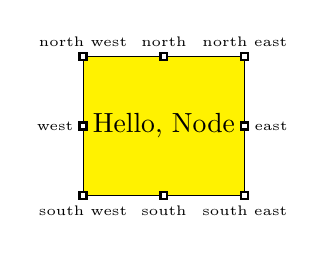
\begin{tikzpicture}
	\node [draw, fill=yellow, minimum size=5em] (hellonode) {Hello, Node};
	\foreach \anchor/\placement in {%
			north/above, north east/above, east/right, south east/below, south/below, south west/below, west/left, north west/above%
	}{%
		\path [draw, thick, fill=white] ([xshift=-0.125em, yshift=-0.125em] hellonode.\anchor) rectangle ++(0.25em, 0.25em);
		\node at (hellonode.\anchor) [font=\tiny, \placement] {\anchor};
	}
\end{tikzpicture}
}
		\only<2>{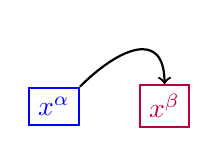
\begin{tikzpicture}
\node at (0em, 0em) [draw, thick, blue]
	(my element A) {$x^\alpha$};
\node at (4em, 0em) [draw, thick, purple]
	(my element B) {$x^\beta$};
\draw [thick, ->] (my element A.north east) ..
	controls ++(45:2em) and ++(90:2em)
	.. (my element B.north);
\end{tikzpicture}
}
	\end{center}%
	\only<2>{\lstinputlisting[firstline=2, lastline=8]{figures/getting-started/node-6}}
\end{frame}

\only<presentation>{
\begin{frame}{A Worked Example}
	We want the following diagram in Ti\emph{k}z, where do we start?!
	\begin{columns}[c]%
		\column{.2\textwidth}%
			\begin{center}%
				\visible<2->{Lines\hspace{.25em}\tikz[na]{\coordinate (label lines);}}
			\end{center}
		\column{.6\textwidth}%
			\begin{center}
				\begin{tikzpicture}[na]
					\pgfdeclareimage[width=.6\textwidth]{spec}{images/simple-spec}
					\node [anchor=south west, text width=.6\textwidth, text height=.729\textwidth, inner sep=0]
						(specification) {\pgfbox[left, bottom]{\pgfuseimage{spec}}};

					% The following line draws a grid for calibration
					% \draw [step=1em] (specification.south west) grid (specification.north east);

					\coordinate (diagram vector) at (3.65em, 5em);
					\coordinate (diagram arc) at (3.5em, 2.8em);
					\coordinate (diagram baseline) at (3.4em, 2.0em);
					\coordinate (diagram opposite) at (6.05em, 7em);

					\coordinate (diagram 2i) at (4em, 1em);
					\coordinate (diagram pio2) at (7.5em, 2.5em);
					\coordinate (diagram 4j) at (7.75em, 6em);
					\coordinate (diagram V) at (3em, 7em);
					\coordinate (diagram theta) at (4.25em, 3.5em);
				\end{tikzpicture}
			\end{center}
		\column{.2\textwidth}%
			\begin{center}%
				\visible<4->{\tikz[na]{\coordinate (label nodes);}\hspace{.5em}Nodes}
			\end{center}
	\end{columns}%

	\begin{tikzpicture}[
		overlay,
		remember picture,
		every path/.style = {ultra thick, ->, draw, uompurple},
		every node/.style = {draw, uomgrey},
	]
		\only<3-4>{
			\draw (label lines.center) to (diagram vector);
			\draw [bend right] (label lines.center) to (diagram arc);
			\draw [bend right] (label lines.center) to (diagram baseline);
			\draw [bend left] (label lines.center) to (diagram opposite);
		}
		\only<5->{
			\node at (diagram 2i) [minimum size=1.85em] (hglt 2i) {};
			\node at (diagram pio2) [minimum size=1.95em] (hglt pio2) {};
			\node at (diagram 4j) [minimum size=2.50em] (hglt 4j) {};
			\node at (diagram theta) [minimum size=1.85em] (hglt theta) {};
			\node at (diagram V) [rotate=63, text width=6em, text height=1.5em] (hglt V) {};

			\foreach \hglt in {2i, pio2, 4j, theta, V}{%
				\draw [bend right, uomgrey] (label nodes.center) to (hglt \hglt);
			}
		}
	\end{tikzpicture}
\end{frame}
}

% \foreach [count=\n] \stage/\fl/\ll in {%
% 	1/1/5, 2/1/8, 3/1/8, 4/2/7, 5/2/7, 6/7/9, 7/7/9, 8/3/7, 9/3/8,
% 	10/3/10, 11/3/10, 12/3/10, 13/11/11, 14/11/14, 15/11/11, 16/11/12,
% 	final/11/14
% }{%
% 	\begin{frame}[plain]{A Worked Example}
% 		\begin{columns}[c]%
% 		\column{.25\textwidth}%
% 			\begin{center}%
% 				\includegraphics[width=\textwidth]{images/simple-spec}
% 				\vspace{1em}
% 			\end{center}
% 		\column{.25\textwidth}%
% 			\begin{center}%
% 				\input{figures/getting-started/example-\stage}
% 			\end{center}
% 		\end{columns}%
% 		\ifthenelse{15=\n}{%
% 			The \texttt{arc} command:\\
% 			\texttt{\textbackslash draw (\ldots) arc ($\alpha$:$\beta$:$r$)}
% 	
% 			An arc of radius $r$ from $\alpha$ to $\beta$.
% 		}{}%
% 		\ifthenelse{17=\n}{%
% 			PGF Math allows us to perform calculations.\\
% 			\texttt{\textbackslash pgfmath\ldots}
% 		}{}%
% 		\lstinputlisting[firstline=\fl, lastline=\ll, numbers=left, firstnumber=\fl]{figures/getting-started/example-\stage}%
% 	\end{frame}
% }

\begin{frame}[plain]{A Worked Example}
	\begin{figure}[htbp]%
		\centering%
		\begin{subfigure}[c]{.25\textwidth}%
			\centering
			\includegraphics[width=\textwidth]{images/simple-spec}
			\vspace{1em}
		\end{subfigure}\only<presentation>{\hspace{.25\textwidth}}%
\foreach [count=\n] \stage/\fl/\ll in {%
	1/1/5, 2/1/8, 3/1/8, 4/2/7, 5/2/7, 6/7/9, 7/7/9, 8/3/7, 9/3/8,
	10/3/10, 11/3/10, 12/3/10, 13/11/11, 14/11/14, 15/11/11, 16/11/12,
	final/11/14
}{%
	\only<\n>{%
		\begin{subfigure}[c]{.25\textwidth}%
			\centering
			\input{figures/getting-started/example-\stage}
		\end{subfigure}
	}%
}%
	\end{figure}%
% 	\ifthenelse{15=\n}{%
% 		The \texttt{arc} command:\\
% 		\texttt{\textbackslash draw (\ldots) arc ($\alpha$:$\beta$:$r$)}
% 
% 		An arc of radius $r$ from $\alpha$ to $\beta$.
% 	}{}%
% 	\ifthenelse{17=\n}{%
% 		PGF Math allows us to perform calculations.\\
% 		\texttt{\textbackslash pgfmath\ldots}
% 	}{}%
\foreach [count=\n] \stage/\fl/\ll in {%
	1/1/5, 2/1/8, 3/1/8, 4/2/7, 5/2/7, 6/7/9, 7/7/9, 8/3/7, 9/3/8,
	10/3/10, 11/3/10, 12/3/10, 13/11/11, 14/11/14, 15/11/11, 16/11/12,
	final/11/14
}{%
	\only<\n>{%
		\lstinputlisting[firstline=\fl, lastline=\ll, numbers=left, firstnumber=\fl]{figures/getting-started/example-\stage}%
	}%
}%
\end{frame}

\begin{frame}[plain]{A Worked Example}
	\lstinputlisting[firstline=3, lastline=18, numbers=left, firstnumber=3]{figures/getting-started/example-final}
\end{frame}

\begin{frame}{A Brief Review}
	\begin{itemize}
		\item Drawing primitives
		\begin{itemize}
			\item Commands and (some) options
			\item Co-ordinate systems
		\end{itemize}
		\item Nodes and Text
		\item A ``Short'' Example (around 15 lines of code)
		\begin{itemize}
			\item Use of primitives
			\item Developing a diagram
			\item Advanced node placement
			\item PGF Math
		\end{itemize}
	\end{itemize}
\end{frame}


\section{More Complicated Examples}
\subsection{Styling TikZ Pictures}
\begin{frame}{The Need for Styling}
	Often have many
	\begin{itemize}
		\item similar elements in diagram (e.g.\ vectors, guidelines)
		\item classes of diagram in document (e.g.\ Petri nets, FSM)
	\end{itemize}
	Don't want to change every one individually!

	Applying styles is good practise.
\end{frame}

\begin{frame}{The Need for Styling}
	In the previous example
	\begin{itemize}
		\item One vector
		\item Two guidelines
	\end{itemize}
	Could have many more -- styles make this easy
\end{frame}

\begin{frame}{Defining Styles}
	Styles define a set of options with one name, created using:
	\begin{description}
		\item[\texttt{\textbackslash tikzstyle}] Easier to use, less useful
		\item[\texttt{\textbackslash tikzset}] Preferred method
	\end{description}

	\texttt{[very thick, blue, ->]} becomes \texttt{[vector]} after
	\lstinputlisting{figures/styling/1}

\end{frame}

\begin{frame}[plain]{Back to the Example}

\end{frame}


\subsection{Animating a Diagram with Beamer}

\section{Finishing Examples}

\section{Conclusion?}

\end{document}
